\subsection{display-worker}

The display-worker is responsible for showing content to users on whatever screen that they are using.
This component must be able to adapt to a variety of different environments, be it the 360 degree
panoramic screen, a wall of giant monitors, or just a user's desktop machine. Additionally, we aim to
have something capable of showing a variety of content, both developed in-house as well as arbitrary
third-party content, allowing for a larger variety of use-cases and usage than some previous art, where
all content had to be built for their environment.

\begin{figure}
    \centering
    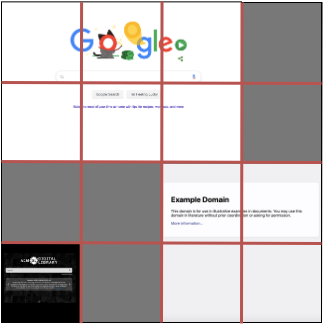
\includegraphics[width=0.5\columnwidth]{chapters/02_technology/figures/display_server.png}
    \caption{Image highlighting grid on display-worker. The red lines are added here for clarity, and are not present in the actual software.}
    \label{fig:cycle-cais}
\end{figure}

To accomplish this, we build off the open-source Electron project, which provides a wrapper around the
Chromium project to build desktop applications. Through this, our content then is displayed as websites
within the display-worker, where the websites can be pointing at localhost applications, or external
sites. The display-worker is set-up such that it provides the user with a N by M grid, where N and M are
configurable beforehand to fit the environment, where a user may open any number of webviews to take
up X by Y rectangle on the grid. Within each webview, we load a website. Webviews may stack upon each
other, and be moved as needed by a user. When dealing with multiple displays, we assume that the displays
are ``continuous'', and share the same dimensions as all other displays within the grid. The grid is then
divided equally amongst all screens.


The display
server is based on our prior work on developing a virtual mouse
interface~\cite{peveler_virtual_2020}, which we quickly describe
here. The server runs an
Electron~\footnote{https://www.electronjs.org/} application, which
provides a chromium based engine to render web content. In the
display, the available screen real estate is divided into a grid,
and then websites are loaded into so-called ``webviews;; that then
takes up some amount of that grid. For example, in Figure
\ref{fig:display_server_grid}, we show a 4x4 grid with 3 open
webviews that take up differing amounts of the grid.

Manipulating the webviews, be it opening / closing them, moving them
around, or resizing them, is done through a REST API that accepts
a JSON object describing the type of change (e.g. open, close), an
ID of the webview if affecting an existing one, and
details on the change (e.g. change size to 2x2, move to 3x4 on grid).
When opening a webview, an additional parameter is accepted that
tells the system whether or not that component exposes a MUIFOLD
mobile UI, and a URL to the JavaScript files necessary to load and
run that UI. Requests to this API can come from the mobile UI or
from an external server unconnected to MUIFOLD. Communication
between the clients and display server happens via WebSockets where
client UIs pass information as to where their current cursor is
as well as potential actions to take (e.g. clicking or scrolling)
which the display server carries out on the webview underneath
the cursor (while leaving all other webviews alone). Through this
separation, clients are able to interact with different webviews
simultaneously if they so choose, or come together on one single
webview.